%--------------------------------------------------
\section{Contexto del sistema}
La clínica cuenta con 12 consultorios para atender a sus pacientes. Dichos pacientes tienen la opción pedir una cita con anticipación para asegurar su atención, o puede presentarse directamente. En este último caso, el paciente puede pasar inmediatamente a consulta sólo si existe un horario libre de un consultorio, o puede pedir una cita para otro día. Al momento de presentarse a su cita, el paciente debe pagar su consulta personalmente.\\

Cada paciente cuenta con un expediente clínico donde se registran sus antecedentes patológicos, historial de consultas, entre otras cosas.\\

También la clínica cuenta con una farmacia encargada de surtir los medicamentos para cada paciente después de haber realizado su consulta.\\


%--------------------------------------------------
\section{Procesos actuales}


% - - - - - - - - - - - - - - - - - - - - - - - - -
\subsection{Participantes}

\begin{itemize}
\item \textbf{Cliente: }Persona que agenda una cita.
\item \textbf{Paciente: }Persona que presenta un malestar o siente la necesidad de ser atendido por un médico.
\item \textbf{Enfermera: }Auxiliar del médico, encargada de agendar citas para los pacientes.
\item \textbf{Médico: }Encargado del diagnóstico de la situación del paciente, se encarga de escribir de su tratamiento y sus controles.
\item \textbf{Cajero: }Encargado de la venta de medicamentos y del cobro de las consultas.
\end{itemize}
\newpage

% - - - - - - - - - - - - - - - - - - - - - - - - -
\subsection{Procesos}

\begin{figure}[htbp!]
		\centering
			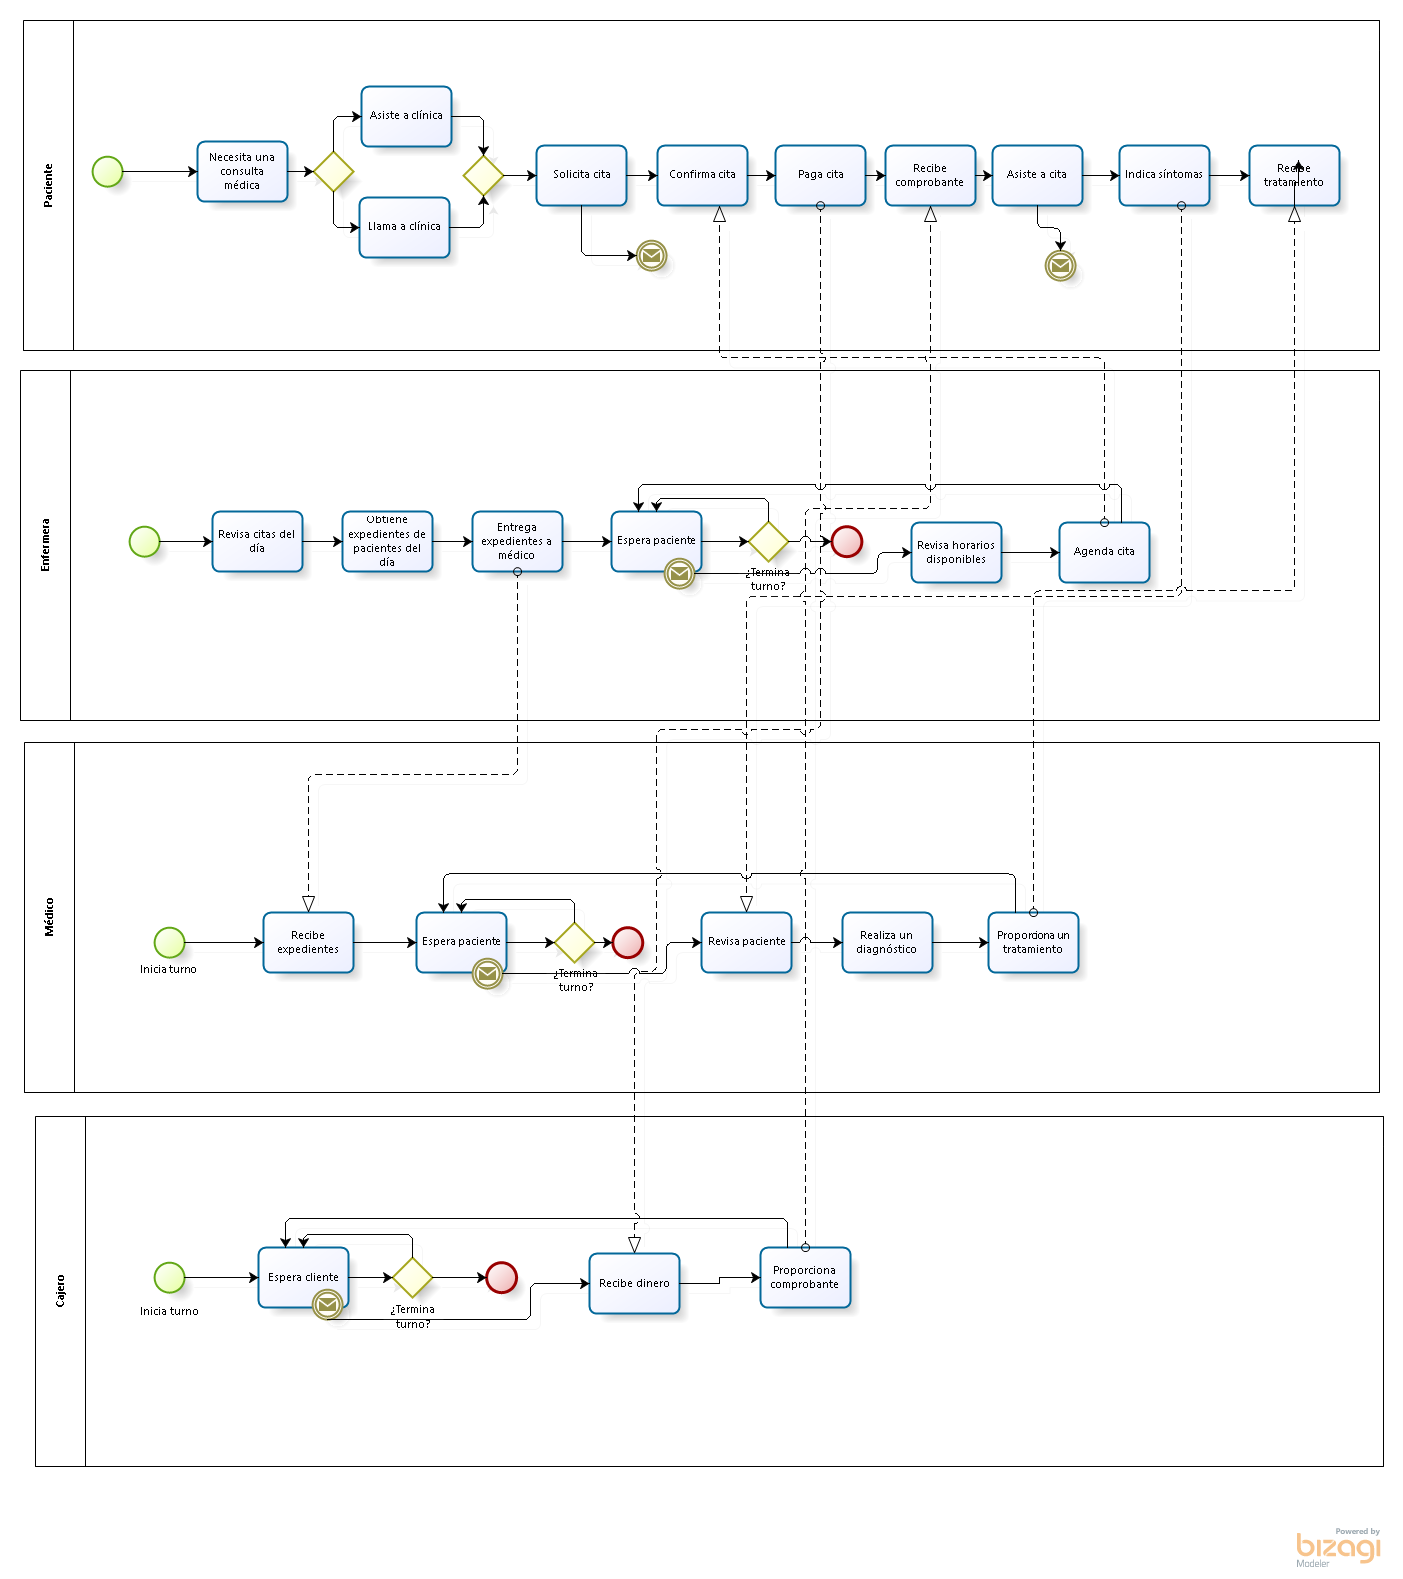
\includegraphics[width=0.8\textwidth]{images/Proceso_actual}
		\caption{Diagrama del proceso actual.}
	\end{figure}

El proceso comienza cuando un paciente presenta la necesidad de que sea atendido por un médico. Para esto, el paciente se presenta directamente en la clínica para poder registrarse mediante una libreta donde se tienen los horarios y consultorios disponibles.\\

Hecho esto, el paciente regresa a su domicilio para esperar a que llegue el dia y hora de la cita. Después el paciente se presenta de nuevo en la clínica 15 minutos antes de la hora de su cita para poder ser recibido y confirmado para su cita, para así poder cubrir el costo de la consulta presentándose directamente con el cajero. Después el paciente espera la hora de su cita para que pueda ser atendido por el médico que se encuentra trabajando en el consultorio asignado en la cita.\\

Después de eso al paciente se le realiza una receta médica que contiene los medicamentos y/o tratamientos que debe de tomar dependiendo del diagnóstico del médico, el cual se almacena una copia en el expediente médico del paciente.\\ 

Finalmente, el paciente opcionalmente se presenta con el cajero para poder ser surtido de sus medicamentos recetados por el médico. En caso de no desear adquirir los medicamentos dentro de la clínica, el paciente los obtiene de lugares externos a la clínica.

%--------------------------------------------------
\section{Problemas identificados}

% - - - - - - - - - - - - - - - - - - - - - - - - -
\subsection{Problema general}

La clínica no cuenta con un control de citas, ni con un control de inventario, mucho menos con un acceso fácil y rápido del historial médico del paciente.

% - - - - - - - - - - - - - - - - - - - - - - - - -
\subsection{Descomposición del problema}

\begin{enumerate}
\item No se cuenta con un registro de las ventas que realiza la farmacia por lo tanto no se sabe el monto total que genera esta parte de la clínica.
\item No existe un control del inventario de la farmacia, por lo que al momento de comprar más medicamentos no se saben las cantidades disponibles ni las diferentes presentaciones de cada medicamento.
\item Se atiende a los pacientes conforme llegan a la clínica.
\item No se cuenta con un control ordenado de citas debido a que hay varias recepcionistas y no tienen un cuaderno de citas común.
\item Las enfermeras pierden tiempo llenando el historial médico del paciente a mano.
\item Se pierde tiempo buscando el historial médico del paciente.
\item El historial médico se daña por el uso que se le da y/o el tiempo que lleva guardado.
\item Los historiales médicos pueden traspapelarse o ser extraviados por el personal.
\item No se cuenta con un registro de citas atendidas. 
\item No se tiene un control para el manejo de los horarios de los consultorios.
\item La información personal de los médicos no se encuentra actualizada porque se pierde el documento que fue llenado o se encuentra en mal estado.
\item El paciente tiene que ir a la clínica físicamente para agendar una cita, con el riesgo de que no haya horarios disponibles causando al paciente una pérdida de su tiempo.
\item La negligencia de las recepcionistas puede afectar el proceso de negocio.
\item Existe duplicidad de expedientes médicos debido a que cuando no se encuentra rápidamente un expediente, el médico se ve en la necesidad de crear uno nuevo para el mismo paciente. 
\item Los pacientes olvidan el horario o el consultorio donde agendaron su cita.
\item Las recepcionistas no cuentan con una forma de avisar a los clientes si su cita fue cancelada o pospuesta. 
\item Si las recepcionistas se encuentran ocupadas el proceso de agendar citas se vuelve lento.
\item El tiempo de la consulta se puede prolongar caso de que el expediente del paciente no esté disponible en el momento.
\item Pueden producirse malentendidos al comprar los medicamentos prescritos en la receta debido a que estas son escritas a mano por el médico.
\item El proceso de llenado de una receta se puede prolongar porque dicha receta actualmente es llenada a mano.
\end{enumerate}
% - - - - - - - - - - - - - - - - - - - - - - - - -
\subsection{Análisis de causas}

\begin{figure}[htbp!]
		\centering
			\includegraphics[width=1\textwidth]{images/Ishikawa}
		\caption{Diagrama de Ishikawa.}
	\end{figure}
    
En la figura 2.2 podemos observar: \\
Personal
\begin{itemize}
	\item Los historiales médicos pueden traspapelarse o ser extraviados por el personal.
    \begin{itemize}
		\item El personal es descuidado.
        \item No se tiene un lugar común para los historiales médicos.
	\end{itemize}
    
    \item Los pacientes olvidan el horario o el consultorio donde agendaron su cita.
	\begin{itemize}
		\item Descuido personal.
	\end{itemize}
    
    \item Las recepcionistas no cuentan con una forma de avisar a los clientes si su cita fue cancelada o pospuesta. 
	\begin{itemize}
		\item El paciente no deja un teléfono actualizado para contactarlo.
	\end{itemize}
    
    \item Si las recepcionistas se encuentran ocupadas el proceso de agendar citas se vuelve lento.
	\begin{itemize}
		\item Tienen más responsabilidades en la clínica.
	\end{itemize}
    
    \item Pueden producirse malentendidos al comprar los medicamentos prescritos en la receta debido a que estas son escritas a mano por el médico.
	\begin{itemize}
		\item El doctor tiene una letra ilegible.  
	\end{itemize}

\end{itemize}

Administración

\begin{itemize}
	\item No se cuenta con un registro de las ventas que realiza la farmacia por lo tanto no se sabe el monto total que genera esta parte de la clínica.
	\begin{itemize}
		\item Se les hace muy difícil llevar un control de ventas escrito a mano porque distintas personas lo manejan.
	\end{itemize}
    
    \item Como no se cuenta con una administración del inventario, se debe buscar visualmente el medicamento en la farmacia, lo cual puede prolongar el proceso de vender medicamentos, lo cual puede afectar el humor de los clientes.

	\begin{itemize}
		\item Se les hace muy difícil llevar un control de inventario escrito a mano porque distintas personas lo manejan.
	\end{itemize}
    
    \item No existe un control del inventario de la farmacia, por lo que al momento de comprar más medicamentos no se saben las cantidades disponibles ni las diferentes presentaciones de cada medicamento.

	\begin{itemize}
		\item no existe un control de inventario porque no se tiene una herramiento para llevarlo de una manera  concurrente con los distintos vendedores. 
	\end{itemize}
    
    \item Existe duplicidad de expedientes médicos debido a que cuando no se encuentra rápidamente un expediente, el médico se ve en la necesidad de crear uno nuevo para el mismo paciente. 
	\begin{itemize}
		\item No se tienen los expedientes en un lugar común.
        \item Los médicos no lo regresan al lugar donde encontraron el expediente.
		\item Olvidan volver a poner el expediente en donde lo encontraron.
	\end{itemize}
    
    \item No se cuenta con un  cuaderno común para tener el control de citas debido a que hay varias recepcionistas; esto genera traslapes de citas, citas duplicadas e incluso un orden diferente para atender a los pacientes.

	\begin{itemize}
		\item Varias recepcionistas trabajando de una manera concurrente.
	\end{itemize}
    
    \item No se tiene un control para el manejo de los horarios de los consultorios.
	\begin{itemize}
		\item Tener los horarios en un cuaderno es poco eficiente(se daña,es ilegible, se piede, etc)
        \item El gerente no siempre se encuentra con tiempo libre para proporcionarle el horario al médico.
	\end{itemize}
\end{itemize}

Proceso
\begin{itemize}
	 \item El tiempo de espera por una cosulta no agendada se puede prolongar mucho afectando el humor de los posibles clientes.
	\begin{itemize}
		\item Existe una gran fila de espera de pacientes sin cita agendada.
	\end{itemize}
    
     \item El registro de citas se hace personalmente o mediante una llamada telefónica, al ser trato de humano a humano existen muchos factores que pueden afectar el proceso de agendar una cita. Ejemplos de factores: Humor,disponibilidad y estado emocional por mencionar algunos.
	\begin{itemize}
		\item Las personas con las que se hace trato para agendar citas son humanos y tienen problemas personales que externan en el trabajo.  
	\end{itemize}
 
     \item El paciente tiene que ir a la clínica físicamente para agendar una cita, con el riesgo de que no haya horarios disponibles causando al paciente una pérdida de su tiempo.

	\begin{itemize}
		\item Existe una gran línea de espera de citas ya agendadas. 
	\end{itemize}
    
    
     \item El proceso de llenado de una receta se puede prolongar porque dicha receta actualmente es llenada a mano.


	\begin{itemize}
		\item La receta es llenada a mano por el médico.
	\end{itemize}
\end{itemize}

Materiales 
\begin{itemize}
	\item Cuando se está creando un expediente nuevo el médico tiene que llenar el expediente a mano, esto genera que no exista un formato único de expedientes.
	\begin{itemize}
		\item La letra, orden de apartados y orden de datos es diferente dependiendo del doctor que lo escriba..
	\end{itemize}

    \item Se pierde tiempo buscando el historial médico del paciente.
	\begin{itemize}
		\item El historial médico no se encuentra en un lugar común para encontrarlo.
        \item Los historiales que sí se encuentran en un lugar común no tienen un orden.
	\end{itemize}
    
    
    \item El historial médico se daña por el uso que se le da y/o el tiempo que lleva guardado.
	\begin{itemize}
		\item El cuidado con el que es tratado el historial no el óptimo. 
		\item El historial lleva mucho tiempo guardado sin un protector.
	\end{itemize}
    
    
    \item Se cuenta con un registro inicial para los médicos pero por tiempo,espacio, uso, el formato de información de médicos se va perdiendo ocasionando la pérdida de información del médico.
	\begin{itemize}
		\item El cuidado con el que son tratados los formatos de información de médico no es cuidadoso.
        \item El formato de información de médico lleva demasiado tiempo guardado.
	\end{itemize}
    
    
    \item El tiempo de la consulta se puede prolongar caso de que el expediente del paciente no esté disponible en el momento.



	\begin{itemize}
		\item Otro médico olvidó regresar el expediente al lugar donde lo encontró.

	\end{itemize}
\end{itemize}
%--------------------------------------------------
\section{Propuesta de solución}

% - - - - - - - - - - - - - - - - - - - - - - - - -
\subsection{Alternativas de solución}
\begin{enumerate}
\item \textbf{Alternativa de solución 1}
\begin{itemize}

\item \textbf{Control de citas: }Llevar el control de citas por medio de una bitácora (cuaderno) ordenada por días y horarios en el cual los pacientes podrán llegar con anticipación a registrar su cita. Se deberá registrar el nombre del médico, el consultorio y el horario; será responsabilidad de las enfermeras llenar dichos registros.\\

\item \textbf{Historial médico del paciente: }Cuando el médico otorgue un tratamiento a un paciente, este deberá usar papel carbón para hacer una copia exacta , la cual servirá para llevar el historial del paciente.\\

\item \textbf{Control de inventario: }En dado caso que el paciente decida comprar el medicamento necesario para su tratamiento, deberá entregar una de las copias al encargado de la caja. El encargado de la caja de la clínica, deberá recibir una de las copias que el medico género para guardarla y deberá marcar aquellos medicamentos y la cantidad de ellos que haya vendido al paciente.\\


\end{itemize}
\item \textbf{Alternativa de solución 2}
\begin{itemize}

\item \textbf{Control de citas: }Llevar el control de citas por medio de documentos de texto (uno para cada consultorio y horario) , en dichos documentos se colocarán tablas con las columnas Médico, Consultorio, Horario. Solo las enfermeras y médicos podrán tener acceso a estos documentos. Si un médico suele estar en más de un consultorio deberá consultar el documento de cada uno de los consultorios.\\

\item \textbf{Historial médico del paciente: }Se tendrán documentos con el registro del tratamiento que el médico haya otorgado a un paciente, el médico creará un nuevo documento del paciente cada que este vaya a una cita, estos documentos se agruparán en carpetas para cada uno de los pacientes. Es importante mencionar que se tendrá una carpeta con registros de un paciente en más de un consultorio, por lo que se recomienda a los pacientes que procuren atenderse en un mismo consultorio. El médico podrá imprimir un tratamiento si el paciente lo requiere, con original y copia del mismo.\\

\item \textbf{Control de inventario: }El paciente otorgará una de las copias al encargado de la farmacia, la cual contendrá sus datos.\\


\end{itemize}
\end{enumerate}

